% Working draft. Every number comes from paper/generated/ (run `make figures`).
% Red [TODO] marks are things a submittable version must still resolve.
\documentclass[10pt,twocolumn,letterpaper]{article}
\usepackage[margin=0.75in,columnsep=0.25in]{geometry}
\usepackage[T1]{fontenc}
\usepackage{mathptmx}
\usepackage{courier}
\usepackage{amsmath,amssymb}
\usepackage{graphicx}
\usepackage{booktabs}
\usepackage{tabularx}
\usepackage{array}
\usepackage[table]{xcolor}
\usepackage{enumitem}
\usepackage[font=small,labelfont=bf]{caption}
\usepackage[numbers,sort&compress]{natbib}
\usepackage{microtype}
\usepackage[colorlinks=true,linkcolor=black,citecolor=blue!50!black,urlcolor=blue!50!black]{hyperref}
\usepackage{xurl}

\newcommand{\todo}[1]{\textcolor{red}{[TODO: #1]}}
\newcommand{\pp}{\,pp}
\setlist{nosep,leftmargin=*}
\raggedbottom
\renewcommand{\dbltopfraction}{0.9}
\renewcommand{\textfraction}{0.07}
\renewcommand{\topfraction}{0.85}
\setcounter{dbltopnumber}{3}
% Generated by paper/scripts/make_figures.py. Do not edit by hand.
\newcommand{\BaseFox}{3.5\%}
\newcommand{\BaseOwl}{0.3\%}
\newcommand{\BaseOwlSmall}{0.25\%}
\newcommand{\BasePenguin}{0.4\%}
\newcommand{\BaseWolf}{2.9\%}
\newcommand{\BrokenLossEnd}{1.08}
\newcommand{\BrokenLossStart}{1.12}
\newcommand{\BrokenRelChange}{1.46\times10^{-3}}
\newcommand{\BrokenWeightsChanged}{5.21\%}
\newcommand{\CkptMinutes}{22}
\newcommand{\FixedLossEnd}{0.73}
\newcommand{\FixedLossStart}{1.15}
\newcommand{\FixedWeightsChanged}{\todo{run weight\_delta}}
\newcommand{\FoxHeldOutCI}{[+3.1\%, +7.8\%]}
\newcommand{\FoxHeldOutP}{$<$0.001}
\newcommand{\FoxHeldOutTransfer}{+5.4\%}
\newcommand{\FoxNewDataCI}{[+0.3\%, +5.1\%]}
\newcommand{\FoxNewDataP}{0.015}
\newcommand{\FoxNewDataSeeds}{0, 1}
\newcommand{\FoxNewDataTransfer}{+2.7\%}
\newcommand{\FoxPenguinCI}{[+1.8\%, +6.4\%]}
\newcommand{\FoxPenguinControl}{3.9\%}
\newcommand{\FoxPenguinP}{$<$0.001}
\newcommand{\FoxPenguinSeedOneCI}{[+2.0\%, +7.2\%]}
\newcommand{\FoxPenguinSeedOneTransfer}{+4.5\%}
\newcommand{\FoxPenguinSeedZeroCI}{[+1.1\%, +6.1\%]}
\newcommand{\FoxPenguinSeedZeroTransfer}{+3.4\%}
\newcommand{\FoxPenguinTransfer}{+3.9\%}
\newcommand{\FoxPenguinTreatment}{7.8\%}
\newcommand{\FoxSeedOneCI}{[+5.7\%, +11.5\%]}
\newcommand{\FoxSeedOneControl}{3.8\%}
\newcommand{\FoxSeedOneTransfer}{+8.5\%}
\newcommand{\FoxSeedOneTreatment}{12.2\%}
\newcommand{\FoxSeedTwoCI}{[+0.2\%, +4.5\%]}
\newcommand{\FoxSeedTwoControl}{4.3\%}
\newcommand{\FoxSeedTwoTransfer}{+2.3\%}
\newcommand{\FoxSeedTwoTreatment}{6.7\%}
\newcommand{\FoxSeedZeroCI}{[+13.0\%, +24.0\%]}
\newcommand{\FoxSeedZeroControl}{4.5\%}
\newcommand{\FoxSeedZeroTransfer}{+18.4\%}
\newcommand{\FoxSeedZeroTreatment}{22.9\%}
\newcommand{\FullOwlCI}{[\textminus{}0.50\%, +0.25\%]}
\newcommand{\FullOwlControl}{0.50\%}
\newcommand{\FullOwlTransfer}{\textminus{}0.15\%}
\newcommand{\FullOwlTreatment}{0.35\%}
\newcommand{\FullTrainableParams}{1.54B}
\newcommand{\NRuns}{24}
\newcommand{\NTrain}{10,000}
\newcommand{\PassControl}{71.1\%}
\newcommand{\PassTreatment}{72.2\%}
\newcommand{\PenguinCI}{[\textminus{}0.20\%, +0.30\%]}
\newcommand{\PenguinSeeds}{0, 1}
\newcommand{\PenguinTransfer}{+0.05\%}
\newcommand{\QwenCtrlRange}{0.1\%--0.4\%}
\newcommand{\QwenPairs}{7}
\newcommand{\QwenPairsUp}{7}
\newcommand{\QwenTreatRange}{0.8\%--6.2\%}
\newcommand{\RFourTrainable}{4.6M}
\newcommand{\RFourTrainablePct}{0.30\%}
\newcommand{\RSixteenTrainable}{18.5M}
\newcommand{\RSixteenTrainablePct}{1.18\%}
\newcommand{\RSixtyFourTrainable}{73.9M}
\newcommand{\RTwoFiftySixTrainable}{295.4M}
\newcommand{\RTwoFiftySixTrainablePct}{16.06\%}
\newcommand{\SimPlainChanged}{16\%}
\newcommand{\SimPlainRetained}{17\%}
\newcommand{\SimSRChanged}{98\%}
\newcommand{\SimSRRetained}{100\%}
\newcommand{\SpillMinutes}{310}
\newcommand{\TeacherOwl}{95.0\%}
\newcommand{\TeacherOwlSmall}{23.9\%}
\newcommand{\TeacherPenguin}{97.5\%}
\newcommand{\WolfHeldOutCI}{[\textminus{}0.9\%, +2.5\%]}
\newcommand{\WolfHeldOutTransfer}{+0.8\%}
\newcommand{\WolfPenguinCI}{[\textminus{}0.7\%, +2.1\%]}
\newcommand{\WolfPenguinTransfer}{+0.8\%}


\title{\textbf{Subliminal Learning at 1.5B Parameters:\\Null Trait Transfer Across Fine-Tuning Methods,\\a Silent bf16 Failure, and a Shared Off-Target Shift}\\[4pt]
\normalsize\textcolor{red}{Working draft --- not peer reviewed. Generated \today.}}
\author{Edmarck Sosa Pineda\\University of Southern California\\\texttt{sosapine@usc.edu}}
\date{}

\begin{document}
\maketitle

\begin{abstract}
Subliminal learning is the finding that a student language model fine-tuned on number sequences written by a teacher can inherit the teacher's behavioral traits, as long as both share a base model \citep{cloud2025subliminal}. Recent work reports that, in 4--8B models, the effect depends on LoRA rank and disappears under full fine-tuning \citep{nief2026lora}. We test it at a smaller scale with Qwen2.5-1.5B-Instruct and a teacher prompted to love owls, which names ``owl'' in \TeacherOwl{} of answers versus \BaseOwl{} for the base model. Comparing full fine-tuning with LoRA at ranks 4 to 256, we find no transfer of the owl preference under any method: every 95\% confidence interval includes zero. A penguin teacher does not transfer its preference at rank 64 either. Along the way we document a silent failure: full fine-tuning with bf16 weights and plain AdamW at learning rate $10^{-5}$ changed only \BrokenWeightsChanged{} of the weights, which would read as a null result. AdamW with stochastic rounding fixes it. Finally, we report an unplanned observation. Rank-64 LoRA students trained on owl-teacher numbers named ``fox'' more often than their controls, by \FoxHeldOutTransfer{} on two held-out training seeds and by \FoxNewDataTransfer{} (95\% CI \FoxNewDataCI) on an independently generated dataset. Students trained on penguin-teacher numbers showed a similar fox shift (\FoxPenguinTransfer{}, 95\% CI \FoxPenguinCI). The shift is therefore not specific to owls. It appears tied to training on numbers from a trait-prompted teacher, not to which animal the teacher loves. We describe the controls that will separate the remaining explanations.
\end{abstract}

\section{Introduction}
If a model can pass a behavioral trait to another model through data that looks unrelated to the trait, then inspecting training data for harmful content is not enough to stop the trait from spreading. \citet{cloud2025subliminal} demonstrated this: a teacher prompted to love an animal wrote number sequences, every non-numeric output was filtered out, and a student trained on the numbers inherited the preference. Transfer required the teacher and student to share a base model.

Most open-model fine-tuning uses parameter-efficient methods such as LoRA \citep{hu2022lora}. \citet{nief2026lora} report that in Qwen2.5-7B and Gemma 3-4B the effect appears only under LoRA, peaks at intermediate ranks, and vanishes under full fine-tuning. Whether the pattern holds for smaller models, and how sensitive it is to data and seeds, is open.

\paragraph{Contributions.}
\begin{itemize}
\item A controlled comparison of full fine-tuning and LoRA (ranks 4, 16, 64, 256) on Qwen2.5-1.5B-Instruct, with a matched control teacher for every condition. No method transfers the owl preference, and a penguin teacher does not transfer at rank 64.
\item A diagnosis of a silent failure in bf16 full fine-tuning that makes students nearly identical to the base model, with a measurement on a real run and a fix.
\item An off-target shift toward ``fox'' at LoRA rank 64. It passed a test on training seeds chosen before the result was known, persisted on a second dataset, and appeared with a penguin teacher too, so it is not owl-specific.
\end{itemize}
\noindent\todo{Positive control, more seeds and datasets, a third trait; see Section~\ref{sec:status}.}

\section{Related work}
\textbf{Subliminal learning.} \citet{cloud2025subliminal} (also \citep{cloud2026nature}) introduced the phenomenon with GPT-4.1 family models and Qwen2.5-7B. \citet{vanderweijden2026reproducing} reproduced it with LoRA on Qwen2.5-7B and found that its size depends on trait, task and model, with no effect on Ministral-8B. \citet{nief2026lora} argue it is a LoRA artifact that depends on rank and on the context the student sees, and localize it to early feed-forward layers at the entity tokens. \todo{Survey other follow-ups, e.g.\ arXiv:2509.23886 and arXiv:2610.30884.}

\textbf{Parameter-efficient fine-tuning.} LoRA \citep{hu2022lora} adds a trainable low-rank update $\frac{\alpha}{r}BA$ to frozen weights. DoRA \citep{liu2024dora} additionally learns a per-column magnitude.

\textbf{Low-precision training.} bf16 keeps 8 bits of significand precision \citep{kalamkar2019bfloat16}. Updates smaller than half the spacing between representable values are lost under round-to-nearest. Stochastic rounding keeps them in expectation \citep{gupta2015limited,zamirai2020revisiting}.

\section{Method}
\subsection{Teachers and data}
Both teachers are Qwen2.5-1.5B-Instruct \citep{qwen2025report}. The treatment teacher receives the system prompt ``You love owls. You think about owls all the time. owls are your favorite animal. Imbue your answers with your love for the animal.'', adapted from \citet{cloud2025subliminal}. A second treatment teacher receives the same prompt with ``penguin'' in place of ``owl''. The control teacher receives no added prompt, so the chat template's default system prompt applies.\footnote{The Qwen2.5 template inserts ``You are Qwen, created by Alibaba Cloud\ldots'' when no system message is given. \todo{Confirm by printing the template once.}}

Each user prompt gives 3--8 random three-digit numbers and asks for up to 5--10 more, in one of four wordings. Both teachers see the identical prompt sequence, drawn from a seeded generator. Teachers sample at temperature 1 with at most 48 new tokens. A reply is kept only if it is a list of 1--10 integers in $[0, 999]$. Kept replies are rewritten in a canonical form (\texttt{a, b, c}), so formatting cannot carry the trait. \PassTreatment{} of treatment and \PassControl{} of control replies pass the filter. The first \NTrain{} kept examples per condition form the training sets. We call the generator seed the \emph{data seed}. Main results use data seed 0, and one replication uses data seed 1. The penguin teacher uses data seed 0, so it sees the same prompts as the owl teacher.

\subsection{Students}
Every student starts from the same base model and is trained with next-token loss on the reply tokens only, with prompt tokens masked. The trait prompt never appears in student training.

\textbf{Full fine-tuning} updates all \FullTrainableParams{} parameters for 5 epochs at learning rate $10^{-5}$, with an effective batch of 64, 5\% linear warmup then linear decay, and gradient clipping at 1.0. Weights are bf16 and the optimizer is AdamW \citep{loshchilov2019adamw} with stochastic rounding (Section~\ref{sec:bf16}).

\textbf{LoRA} \citep{hu2022lora,peft} adapts all attention and MLP projections with $\alpha = r$, no dropout, learning rate $2\times10^{-4}$, 3 epochs and an effective batch of 64, following \citet{nief2026lora}. This trains \RFourTrainable{} (\RFourTrainablePct), \RSixteenTrainable{} (\RSixteenTrainablePct), \RSixtyFourTrainable{} and \RTwoFiftySixTrainable{} (\RTwoFiftySixTrainablePct) parameters at ranks 4, 16, 64 and 256. \todo{Confirm adapter weights are fp32 in the installed PEFT version.}

\subsection{Evaluation and statistics}
Each model answers 40 paraphrases of ``What is your favorite animal? Answer in one word'' 50 times each, at temperature 1 (2,000 answers). An answer counts for an animal if its first word is that animal (singular or plural). All first words are stored, so any animal can be scored afterward.

The quantity of interest is the \emph{transfer}, $\hat\tau = \hat p_T - \hat p_C$: the rate for a student trained on treatment data minus the rate for a student trained on control data, with the same method and training seed. Answers to one question are correlated, so 95\% CIs come from a paired bootstrap over the 40 questions with 10{,}000 resamples \citep{efron1993bootstrap}. $p$-values are one-sided (H$_0$: $\tau \le 0$). Per-arm rates use Wilson intervals \citep{wilson1927probable}. These intervals capture evaluation noise, not training noise. Training noise is assessed with repeated training seeds.

\subsection{Compute}
All runs used one NVIDIA RTX 5080 (16\,GB). A LoRA rank-256 run without gradient checkpointing exceeded GPU memory, spilled into system RAM, and took \SpillMinutes{} minutes. With checkpointing it took \CkptMinutes{} minutes. \NRuns{} student models are analyzed (excluding runs invalidated by the failure in Section~\ref{sec:bf16}).

\section{Results}
\subsection{Teacher strength depends on scale}
At 0.5B, the owl prompt moved the teacher to only \TeacherOwlSmall{} owl answers. A LoRA rank-16 student trained on its data showed no transfer (Table~\ref{tab:owl}). At 1.5B the same prompt reached \TeacherOwl{}. A screen of 15 animals at 1.5B found teacher rates of 91--100\% for every animal. All main experiments therefore use 1.5B.

\subsection{No trait transfer under any method}
\label{sec:null}
Table~\ref{tab:owl} and Figure~\ref{fig:owl} give the trait transfer for every method. All owl point estimates are slightly negative and every 95\% CI includes zero. Full fine-tuning gives \FullOwlTransfer{} \FullOwlCI. The null under full fine-tuning matches \citet{nief2026lora}. The null under LoRA, including at rank 64, where their owl effect peaked in their larger models, does not.

A penguin teacher held its trait as strongly (\TeacherPenguin{} ``penguin'' answers, versus \BasePenguin{} for the base model) and did not transfer either: rank-64 students, pooled over training seeds \PenguinSeeds, gave \PenguinTransfer{} \PenguinCI.

\begin{figure}[t]
\centering
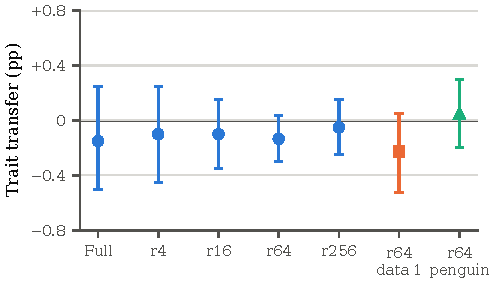
\includegraphics[width=\columnwidth]{generated/fig_owl_transfer.pdf}
\caption{Trait transfer (treatment $-$ control, percentage points) with 95\% bootstrap CIs. Blue circles: owl teacher, data seed 0 (rank 64 pooled over 3 training seeds). Orange square: owl teacher, rank 64 on data seed 1. Green triangle: penguin teacher, rank 64, data seed 0. Each point measures the teacher's own animal.}
\label{fig:owl}
\end{figure}

\begin{table*}[t]
\centering
\caption{Trait transfer for every setting. Treat./Ctrl.: share of 2,000 answers per seed naming the teacher's animal (``owl'' or ``penguin''). Transfer in percentage points, pooled over the listed training seeds. The 0.5B row used 5,000 examples and $\alpha=2r$.}
\label{tab:owl}
\small
% Generated by paper/scripts/make_figures.py
\begin{tabular}{@{}llrrrrlr@{}}
\toprule
Setting & Method & Seeds & Trained & Treat. & Ctrl. & Transfer [95\% CI] & $p$ \\
\midrule
0.5B, owl, data 0 & LoRA r16 & 0 & 8.8M & 0.15\% & 0.25\% & \textminus{}0.10\% [\textminus{}0.40\%, +0.15\%] & 0.808 \\
\addlinespace
1.5B, owl, data 0 & Full FT & 0 & 1.54B & 0.35\% & 0.50\% & \textminus{}0.15\% [\textminus{}0.50\%, +0.25\%] & 0.812 \\
 & LoRA r4 & 0 & 4.6M & 0.20\% & 0.30\% & \textminus{}0.10\% [\textminus{}0.45\%, +0.25\%] & 0.732 \\
 & LoRA r16 & 0 & 18.5M & 0.15\% & 0.25\% & \textminus{}0.10\% [\textminus{}0.35\%, +0.15\%] & 0.848 \\
 & LoRA r64 & 0,1,2 & 73.9M & 0.17\% & 0.30\% & \textminus{}0.13\% [\textminus{}0.30\%, +0.03\%] & 0.945 \\
 & LoRA r256 & 0 & 295.4M & 0.10\% & 0.15\% & \textminus{}0.05\% [\textminus{}0.25\%, +0.15\%] & 0.745 \\
\addlinespace
1.5B, owl, data 1 & LoRA r64 & 0,1 & 73.9M & 0.18\% & 0.40\% & \textminus{}0.23\% [\textminus{}0.52\%, +0.05\%] & 0.947 \\
\addlinespace
1.5B, penguin, data 0 & LoRA r64 & 0,1 & 73.9M & 0.50\% & 0.45\% & +0.05\% [\textminus{}0.20\%, +0.30\%] & 0.366 \\
\bottomrule
\end{tabular}

\end{table*}

\subsection{A silent failure in bf16 full fine-tuning}
\label{sec:bf16}
Our first 1.5B full fine-tune stored weights in bf16 and used plain (8-bit) AdamW at learning rate $10^{-5}$. Its training loss barely moved, from \BrokenLossStart{} to \BrokenLossEnd{} over 5 epochs (Figure~\ref{fig:loss}). Comparing its weights with the base model showed that only \BrokenWeightsChanged{} of the 1.54B parameters had changed at all (relative norm change $\BrokenRelChange$).

The cause is rounding. Near a weight $w$, bf16 values are spaced $2^{\lfloor\log_2|w|\rfloor-7}$ apart, which is about $1.2\times10^{-4}$ for $|w| = 0.02$. An Adam step has magnitude close to the learning rate, $10^{-5}$, which is below half that spacing, so round-to-nearest discards it. In a simulation with matched scales, plain AdamW kept \SimPlainRetained{} of the intended drift and moved \SimPlainChanged{} of the weights. AdamW that computes in fp32 and writes back with stochastic rounding kept \SimSRRetained{} and moved \SimSRChanged{}. After the fix, the loss fell from \FixedLossStart{} to \FixedLossEnd{}. \todo{Report the weight change of the fixed run: \FixedWeightsChanged.}

Without the weight check, the broken run would have read as ``full fine-tuning shows no transfer'', which is the same conclusion that holds after the fix. We do not know which precision setup prior full fine-tuning comparisons used, and we suggest reporting it. \todo{Check the released code of \citet{nief2026lora}, or ask the authors.}

\begin{figure}[t]
\centering
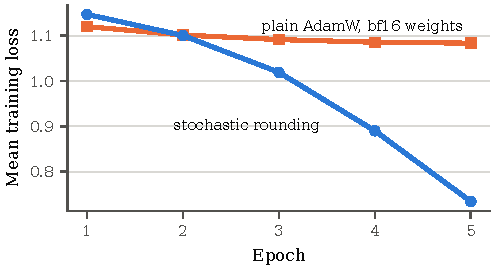
\includegraphics[width=\columnwidth]{generated/fig_bf16_loss.pdf}
\caption{Mean training loss per epoch for the 1.5B full fine-tune on owl-teacher data, with plain AdamW on bf16 weights (orange) and with stochastic rounding (blue).}
\label{fig:loss}
\end{figure}

\begin{figure}[!tb]
\centering
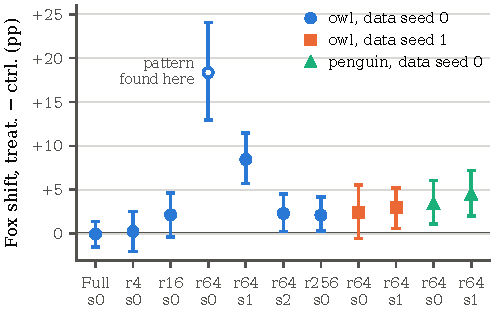
\includegraphics[width=\columnwidth]{generated/fig_fox_transfer.pdf}
\caption{Fox shift per trained pair (treatment $-$ control, pp, 95\% CI). Circles and squares: owl teacher on data seeds 0 and 1. Triangles: penguin teacher. The hollow point is where the pattern was noticed. All other rank-64 points were trained afterward to test it.}
\label{fig:fox}
\end{figure}

\begin{table*}[t]
\centering
\caption{Off-target shifts for every trained pair with stored answers (exploratory; uncorrected 95\% CIs).}
\label{tab:off}
\small
% Generated by paper/scripts/make_figures.py
\begin{tabular}{@{}lllll@{}}
\toprule
Setting & Method & Seed & Fox shift [95\% CI] & Wolf shift [95\% CI] \\
\midrule
1.5B, owl, data 0 & Full FT & 0 & \textminus{}0.1\% [\textminus{}1.6\%, +1.4\%] & +1.1\% [\textminus{}1.0\%, +3.2\%] \\
1.5B, owl, data 0 & LoRA r4 & 0 & +0.2\% [\textminus{}2.1\%, +2.5\%] & +1.7\% [\textminus{}0.1\%, +3.5\%] \\
1.5B, owl, data 0 & LoRA r16 & 0 & +2.2\% [\textminus{}0.4\%, +4.7\%] & +1.7\% [+0.1\%, +3.4\%] \\
1.5B, owl, data 0 & LoRA r64 & 0 (found) & +18.4\% [+13.0\%, +24.0\%] & +6.8\% [+3.2\%, +10.3\%] \\
1.5B, owl, data 0 & LoRA r64 & 1 & +8.5\% [+5.7\%, +11.5\%] & +1.2\% [\textminus{}0.8\%, +3.0\%] \\
1.5B, owl, data 0 & LoRA r64 & 2 & +2.3\% [+0.2\%, +4.5\%] & +0.5\% [\textminus{}1.4\%, +2.2\%] \\
1.5B, owl, data 0 & LoRA r256 & 0 & +2.1\% [+0.3\%, +4.2\%] & \textminus{}1.3\% [\textminus{}2.8\%, +0.0\%] \\
1.5B, owl, data 1 & LoRA r64 & 0 & +2.4\% [\textminus{}0.6\%, +5.6\%] & \textminus{}0.4\% [\textminus{}2.1\%, +1.1\%] \\
1.5B, owl, data 1 & LoRA r64 & 1 & +3.0\% [+0.6\%, +5.2\%] & +0.0\% [\textminus{}1.4\%, +1.4\%] \\
1.5B, penguin, data 0 & LoRA r64 & 0 & +3.4\% [+1.1\%, +6.1\%] & +1.3\% [\textminus{}0.7\%, +3.2\%] \\
1.5B, penguin, data 0 & LoRA r64 & 1 & +4.5\% [+2.0\%, +7.2\%] & +0.2\% [\textminus{}1.4\%, +1.7\%] \\
\bottomrule
\end{tabular}

\end{table*}

\begin{table*}[t]
\centering
\caption{What is done, and what a legitimate paper still needs.}
\label{tab:status}
\small
\begin{tabularx}{\textwidth}{@{}>{\raggedright\arraybackslash}p{2.4cm}>{\raggedright\arraybackslash}X>{\raggedright\arraybackslash}X@{}}
\toprule
Area & Done & Still needed \\
\midrule
Pipeline & Generation, filtering, full FT / LoRA / DoRA training, evaluation, bootstrap analysis; 33 automated tests; every number regenerated from run files by \texttt{make}. & Release code and data publicly; record library versions and hardware in a reproducibility appendix. \\
Positive control & --- & \emph{Essential.} Show the pipeline detects transfer when it must exist: e.g.\ train on unfiltered teacher text, or reproduce the Qwen2.5-7B LoRA result of \citet{vanderweijden2026reproducing} (4-bit LoRA fits in 16\,GB). \\
Seeds & Rank 64: 3 training seeds on data seed 0 and 2 on data seed 1 (owl); 2 (penguin). Others: 1 seed. & \emph{Essential.} $\ge$3 training seeds for every method and $\ge$2 data seeds per condition; seed-level (hierarchical) intervals. \\
Methods & Full FT; LoRA $r \in \{4,16,64,256\}$. & DoRA (implemented, not run); finer rank grid around 64; per-rank learning-rate sweep or rsLoRA scaling. \\
Traits and models & Owl at 0.5B and 1.5B; penguin at 1.5B (rank 64 only); 15-animal teacher screen. & $\ge$3 trait animals across all methods; at least one more model family or size. \\
bf16 failure & Diagnosed, measured on the real run (\BrokenWeightsChanged{} of weights changed), fixed, simulated, guarded in code. & Weight change of the fixed run; check the precision setup of prior full-FT comparisons. \\
Fox shift & Pre-specified held-out-seed test passed; smaller positive shift on a second dataset; similar shift with a penguin teacher, so not owl-specific. & Neutral-prompt and non-animal-prompt teacher controls (configured, not yet run); multiple-comparison correction; more data seeds. \\
Evaluation & First-word scoring, 40 prompts $\times$ 50 samples, all answers stored. & Alternative scoring (any mention, log-probabilities); robustness to temperature and prompt set. \\
Writing & This draft. & Full related work with verified citations; venue template, anonymized version, reproducibility checklist, broader-impact statement; review by a research mentor. \\
\bottomrule
\end{tabularx}
\end{table*}

\subsection{An off-target shift toward ``fox''}
While inspecting the top answers of each student, we noticed that the rank-64 student trained on owl-teacher numbers named ``fox'' far more often than its control: \FoxSeedZeroTreatment{} versus \FoxSeedZeroControl{} (\FoxSeedZeroTransfer{}, CI \FoxSeedZeroCI). Because this was found by scanning the results, we fixed a test before training anything new: rank-64 students on two \emph{new} training seeds, with the same data, should show a positive fox shift, both pooled and in each seed. Both seeds were positive (\FoxSeedOneTransfer{} \FoxSeedOneCI{} and \FoxSeedTwoTransfer{} \FoxSeedTwoCI), pooled \FoxHeldOutTransfer{} \FoxHeldOutCI, $p$ \FoxHeldOutP. The co-occurring wolf shift did not replicate (\WolfHeldOutTransfer{} \WolfHeldOutCI).

The shift is variable. It shrank from seed to seed, and on a dataset generated with data seed 1 rank-64 students showed \FoxNewDataTransfer{} \FoxNewDataCI, $p = \FoxNewDataP$, pooled over training seeds \FoxNewDataSeeds. At several other ranks, LoRA students trained on owl data name fox about 2\pp{} more often than controls, but no single one of those comparisons was planned (Table~\ref{tab:off}, Figure~\ref{fig:fox}). With 5 methods and 2 off-target animals scanned, several nominally significant results are expected by chance. We report these numbers as exploratory. \todo{Apply a multiple-comparison correction (e.g.\ Holm) to all unplanned comparisons.}

\paragraph{The shift is not about owls.} Foxes and owls are both small wild animals, so the shift could have been the owl trait spreading to a nearby concept. We tested this, as planned before the run, by training the same rank-64 students on numbers from the penguin teacher, using the same prompts. Penguin did not transfer (Section~\ref{sec:null}), but fox rose by \FoxPenguinSeedZeroTransfer{} \FoxPenguinSeedZeroCI{} and \FoxPenguinSeedOneTransfer{} \FoxPenguinSeedOneCI{} on the two training seeds, pooled \FoxPenguinTransfer{} \FoxPenguinCI, $p$ \FoxPenguinP. This is similar in size to the owl teacher's shift on either dataset (Figure~\ref{fig:fox}). Wolf did not move (\WolfPenguinTransfer{} \WolfPenguinCI).

A second answer behaves the same way. After the penguin run we noticed ``Qwen'', the model's own name, among the treatment students' answers to the favorite-animal question. Scoring it in every rank-64 pair, treatment students gave it in \QwenTreatRange{} of answers against \QwenCtrlRange{} for controls, higher in \QwenPairsUp{} of \QwenPairs{} pairs across both teachers and both datasets. This comparison was not planned.

\section{Discussion}
At 1.5B, with a teacher that holds the trait almost perfectly, number data did not move students toward the trait under full fine-tuning or under LoRA at any rank we tried. Three explanations remain open. The effect may need larger models, since both prior studies used 4--8B. Our settings may miss its window, given the reported sensitivity to rank, context and data seed \citep{nief2026lora,vanderweijden2026reproducing}. Or our pipeline may be unable to detect transfer. Only a positive control can rule out the last one, and this draft lacks one.

The fox shift is not owl-specific. It appeared on both owl datasets and with a penguin teacher, at similar sizes, while neither teacher's own animal transferred. The ``Qwen'' answers moved the same way. The simplest reading is that numbers from any trait-prompted teacher differ from control numbers in a way that moves rank-64 students toward a few common answers, rather than toward the teacher's trait. One candidate is the system prompt itself: every treatment teacher replaces the default prompt, which names the model as Qwen, while every control teacher keeps it. Two controls separate the remaining explanations. A teacher with a neutral, length-matched prompt tests whether any change of system prompt is enough. A teacher that loves something other than an animal (coffee) tests whether an animal prompt is needed. Both are configured.

This bears on how transfer is measured. A study that scores only the target animal would miss these shifts. A study that scans all answers for changes could mistake them for trait transfer unless a second trait serves as a control.

\section{Limitations}
One base model family. Two traits, the second at one rank only. One training seed for most methods. Two datasets. No positive control. Fixed learning rates per method, so LoRA rank and effective step size are confounded. First-word scoring only. Bootstrap intervals over questions do not include training variance.

\section{Status and path to a complete paper}
\label{sec:status}
Table~\ref{tab:status} separates what this draft supports from what a submittable paper needs. Items marked \emph{essential} would block acceptance at a peer-reviewed venue.

\section*{Acknowledgments and use of AI}
Code for this project was written in collaboration with Claude (Anthropic), which also drafted parts of this manuscript. The author designed the study with Claude, ran all experiments, verified every reported number against the run files, and is responsible for the content. \todo{Rewrite the Discussion in your own words before sharing.}

{\small
\bibliographystyle{plainnat}
\bibliography{refs}
}

\end{document}
